\section{FDE Device-Level Mode Analysis}
The FDE stage resolves the waveguide cross-section and extracts the modal effective index and group index. The target SOI geometry is a silicon core of width \SI{400}{\nano\metre} and height \SI{200}{\nano\metre} on silicon dioxide, as shown in Fig.~\ref{fig:soi-cross-section}. The intended operating mode is the fundamental TE-like mode. A correct FDE study should verify the material mesh, boundary conditions, modal confinement, \(n_{\mathrm{eff}}\), and \(n_g\) near \SI{1550}{\nano\metre}.

\begin{figure}[H]
\centering
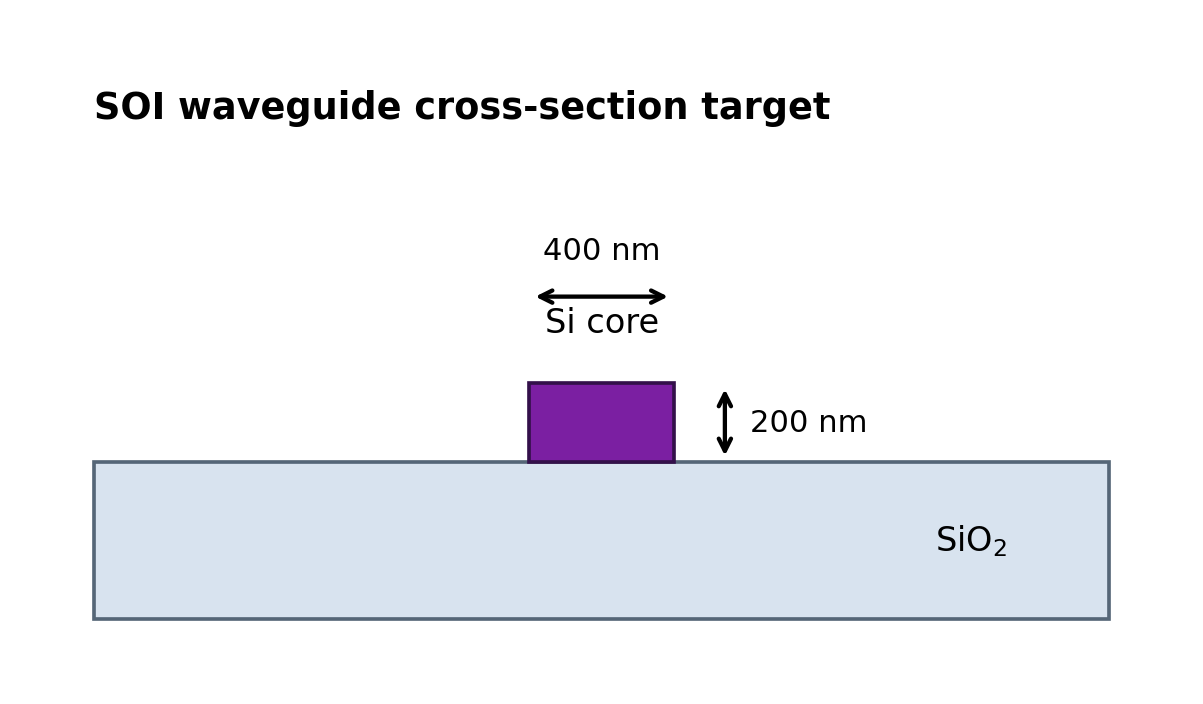
\includegraphics[width=0.72\linewidth]{figures/soi_cross_section_schematic.png}
\caption{Target SOI waveguide cross-section used for the FDE design stage. This schematic is based on the design target and is not an FDE mesh image.}
\label{fig:soi-cross-section}
\end{figure}

No FDE-exported mode profile, effective-index table, group-index table, or mesh image was present in the available \path{results/} or \path{figures/} directories. The original Lumerical MODE file \path{models_original/ring_resonator_studentv2_fde.lms} is available locally but was not modified or included in the Overleaf package.

Using Eq.~\eqref{eq:ring-design}, the ring length required for the target FSR can be written in terms of the unavailable FDE group index:
\begin{equation}
L = \frac{(\SI{1.55}{\micro\metre})^2}{n_g(\SI{0.0262}{\micro\metre})}
  = \frac{\SI{91.70}{\micro\metre}}{n_g},
\end{equation}
\begin{equation}
r = \frac{L}{2\pi}
  = \frac{\SI{14.59}{\micro\metre}}{n_g}.
\end{equation}
These expressions should be evaluated after extracting \(n_g\) at \SI{1550}{\nano\metre} from FDE. A numerical radius is not reported here because no real \(n_g\) value was available.

\begin{table}[H]
\centering
\caption{FDE outputs required for final design completion.}
\label{tab:fde-results}
\begin{tabular}{lll}
\toprule
Quantity & Value & Status \\
\midrule
\(n_{\mathrm{eff}}\) at \SI{1550}{\nano\metre} & TODO & Not available from current simulation output \\
\(n_g\) at \SI{1550}{\nano\metre} & TODO & Not available from current simulation output \\
TE mode confinement & TODO & Not available from current simulation output \\
Boundary condition check & TODO & Not available from current simulation output \\
Ring round-trip length \(L\) & \(\SI{91.70}{\micro\metre}/n_g\) & Target-derived expression \\
Ring radius \(r\) & \(\SI{14.59}{\micro\metre}/n_g\) & Target-derived expression \\
\bottomrule
\end{tabular}
\end{table}
